\documentclass{standalone}
\usepackage{tikz}
\usetikzlibrary{arrows.meta}
\begin{document}
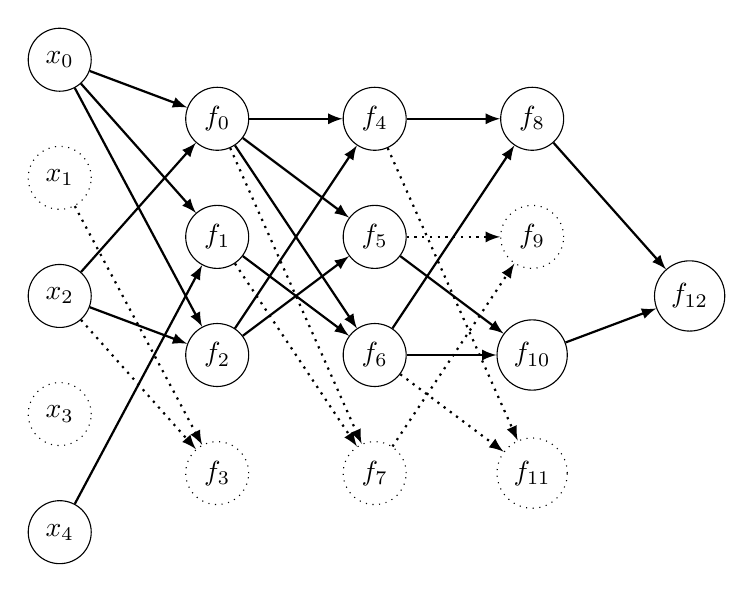
\begin{tikzpicture}[]

\begin{scope}[every node/.style={circle, draw, minimum size=8mm}]
\node (x0) at (0, 0.0) {$x_0$};
\node (x1) at (0, -1.5) [dotted] {$x_1$};
\node (x2) at (0, -3.0) {$x_2$};
\node (x3) at (0, -4.5) [dotted] {$x_3$};
\node (x4) at (0, -6.0) {$x_4$};
\node (f0) at (2.0, -0.75) {$f_{0}$};
\node (f1) at (2.0, -2.25) {$f_{1}$};
\node (f2) at (2.0, -3.75) {$f_{2}$};
\node (f3) at (2.0, -5.25) [dotted] {$f_{3}$};
\node (f4) at (4.0, -0.75) {$f_{4}$};
\node (f5) at (4.0, -2.25) {$f_{5}$};
\node (f6) at (4.0, -3.75) {$f_{6}$};
\node (f7) at (4.0, -5.25) [dotted] {$f_{7}$};
\node (f8) at (6.0, -0.75) {$f_{8}$};
\node (f9) at (6.0, -2.25) [dotted] {$f_{9}$};
\node (f10) at (6.0, -3.75) {$f_{10}$};
\node (f11) at (6.0, -5.25) [dotted] {$f_{11}$};
\node (f12) at (8, -3.0) {$f_{12}$};
\end{scope}
\begin{scope}[-latex, thick]
\draw (x2) -- (f0);
\draw (x0) -- (f0);
\draw (x0) -- (f1);
\draw (x4) -- (f1);
\draw (x2) -- (f2);
\draw (x0) -- (f2);
\draw [dotted] (x1) -- (f3);
\draw [dotted] (x2) -- (f3);
\draw (f0) -- (f4);
\draw (f2) -- (f4);
\draw (f0) -- (f5);
\draw (f2) -- (f5);
\draw (f1) -- (f6);
\draw (f0) -- (f6);
\draw [dotted] (f1) -- (f7);
\draw [dotted] (f0) -- (f7);
\draw (f6) -- (f8);
\draw (f4) -- (f8);
\draw [dotted] (f7) -- (f9);
\draw [dotted] (f5) -- (f9);
\draw (f5) -- (f10);
\draw (f6) -- (f10);
\draw [dotted] (f4) -- (f11);
\draw [dotted] (f6) -- (f11);
\draw(f8) -- (f12);
\draw(f10) -- (f12);
\end{scope}

\end{tikzpicture}
\end{document}

